\documentclass[11pt,a4paper]{article}

% ============ PACKAGES ============
\usepackage[utf8]{inputenc}
\usepackage[T1]{fontenc}
\usepackage[margin=1in]{geometry}
\sloppy
\usepackage{amsmath,amssymb,amsthm}
\usepackage{booktabs}
\usepackage{array}
\usepackage{enumitem}
\usepackage{fancyhdr}
\usepackage{hyperref}
\usepackage{xcolor}
\usepackage{tcolorbox}
\tcbuselibrary{breakable}
\usepackage{float}
\usepackage{listings}
\usepackage{tikz}
\usetikzlibrary{shapes.geometric, arrows.meta, positioning, fit}

% ============ COLORS ============
\definecolor{codeblue}{rgb}{0.13,0.29,0.53}
\definecolor{passgreen}{rgb}{0,0.5,0}
\definecolor{failred}{rgb}{0.8,0,0}
\definecolor{codegray}{rgb}{0.5,0.5,0.5}
\definecolor{backcolour}{rgb}{0.97,0.97,0.97}
\definecolor{notebg}{rgb}{0.93,0.95,1.0}
\definecolor{noteborder}{rgb}{0.4,0.5,0.7}
\definecolor{warningbg}{rgb}{1.0,0.97,0.88}
\definecolor{warningborder}{rgb}{1.0,0.6,0.0}
\definecolor{scenariobg}{rgb}{0.95,1.0,0.95}
\definecolor{scenarioborder}{rgb}{0.2,0.6,0.3}
\definecolor{criticalbg}{rgb}{1.0,0.92,0.92}
\definecolor{criticalborder}{rgb}{0.8,0.2,0.2}
\definecolor{medicalbg}{rgb}{0.95,0.98,1.0}
\definecolor{medicalborder}{rgb}{0.2,0.4,0.8}

% ============ THEOREM ENVIRONMENTS ============
\theoremstyle{definition}
\newtheorem{definition}{Definition}[section]
\newtheorem{invariant}{Invariant}[section]

% ============ BOXES ============
\newtcolorbox{notebox}{
    colback=notebg, colframe=noteborder, boxrule=1pt,
    left=6pt, right=6pt, top=6pt, bottom=6pt
}

\newtcolorbox{warningbox}[1][Warning]{
    colback=warningbg, colframe=warningborder, boxrule=1.5pt,
    left=6pt, right=6pt, top=6pt, bottom=6pt,
    fonttitle=\bfseries, title={#1}
}

\newtcolorbox{criticalbox}[1][Critical]{
    colback=criticalbg, colframe=criticalborder, boxrule=1.5pt,
    left=6pt, right=6pt, top=6pt, bottom=6pt,
    fonttitle=\bfseries, title={#1}
}

\newtcolorbox{scenariobox}[1][Worked Scenario]{
    colback=scenariobg, colframe=scenarioborder, boxrule=1.5pt,
    left=8pt, right=8pt, top=8pt, bottom=8pt,
    fonttitle=\bfseries, title={#1}, breakable
}

\newtcolorbox{medicalbox}[1][Medical Protocol]{
    colback=medicalbg, colframe=medicalborder, boxrule=2pt,
    left=8pt, right=8pt, top=8pt, bottom=8pt,
    fonttitle=\bfseries, title={#1}
}

% ============ CODE STYLE ============
\lstdefinestyle{pythonstyle}{
    backgroundcolor=\color{backcolour},
    basicstyle=\ttfamily\footnotesize,
    keywordstyle=\color{codeblue}\bfseries,
    commentstyle=\color{passgreen},
    breaklines=true, frame=single, numbers=left, numbersep=5pt
}
\lstset{style=pythonstyle}

% ============ HEADERS ============
\pagestyle{fancy}
\fancyhf{}
\fancyhead[L]{\textit{EFM Codex --- Appendix K}}
\fancyhead[R]{\thepage}

% ============ HYPERREF ============
\hypersetup{
    colorlinks=true, linkcolor=codeblue, urlcolor=cyan,
    pdftitle={EFM Codex Appendix K: Systemic Health Sovereignty Layer},
}

% ============ DOCUMENT ============
\title{
    \textbf{\LARGE EFM Codex --- Appendix K}\\[0.3cm]
    \large Systemic Health Sovereignty Layer (SHSL)\\[0.2cm]
    \textit{Capsule Medicine: Diagnosis, Treatment, and Recovery}
}
\author{Entropica SPC --- Yology Research Division}
\date{Version 1.4 --- December 2025}

\begin{document}
\maketitle

\begin{medicalbox}[The Medical Paradigm]
The Systemic Health Sovereignty Layer treats \textbf{malfunction as pathology, not crime}. While Reflex and Arbiter layers enforce rules and resolve conflicts, SHSL enables \textit{proactive recovery} through diagnosis, treatment, and restoration of capsule health.

Not all errors are adversarial. Drift, aging, and memory decay require \textbf{medicine}, not punishment.
\end{medicalbox}

\begin{warningbox}[Volume Dependencies]
This appendix assumes familiarity with:
\begin{itemize}
    \item \textbf{Volume I} --- Entropy ($S$), Reflex Engine
    \item \textbf{Volume II} --- Arbiter Layer, Forest Layer, DDI
    \item \textbf{Appendix A} --- Forensic State Snapshots
    \item \textbf{Appendix F} --- Escalation Protocols
    \item \textbf{Appendix G} --- Gardener Interface
    \item \textbf{Appendix H} --- Telemetry Layer
    \item \textbf{Appendix I} --- Deployment Profiles
\end{itemize}
\end{warningbox}

\tableofcontents
\newpage

% ============ SECTION 1 ============
\section{Overview and Purpose}

\subsection{Why AI Needs a Health Layer}

In distributed AI swarms:
\begin{itemize}
    \item Not all errors are adversarial (drift, aging, memory rot)
    \item Capsules may decay in performance without breaking rules
    \item Reactive halts are expensive; preventive care is cheaper
    \item Recovery preserves capsule knowledge and lineage value
\end{itemize}

\begin{notebox}
\textbf{SHSL Principle:} The health layer operates \textit{orthogonally} to Reflex and Arbiter. It does not replace safety enforcement---it complements it with proactive monitoring and restoration capabilities.
\end{notebox}

\subsection{Design Goals}

\begin{enumerate}
    \item Enable autonomous diagnosis of capsule health anomalies
    \item Provide graduated treatment protocols (soft to invasive)
    \item Preserve capsule autonomy through consent mechanisms
    \item Integrate with existing safety infrastructure (Reflex, Arbiter, Telemetry)
    \item Maintain forensic accountability for all medical interventions
\end{enumerate}

%==============================================================================
% SHSL SYNC DIAGRAM (Design Team Request)
%==============================================================================
\subsection{SHSL Synchronization Architecture}

\begin{figure}[H]
\centering
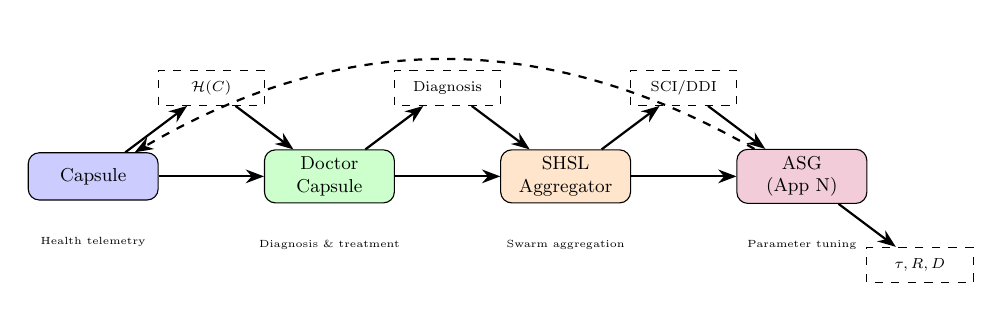
\begin{tikzpicture}[scale=0.75, transform shape,
    node distance=1.2cm,
    component/.style={rectangle, rounded corners, draw, minimum width=2.2cm, minimum height=0.8cm, align=center, font=\small},
    data/.style={rectangle, draw, dashed, minimum width=1.8cm, minimum height=0.6cm, align=center, font=\scriptsize},
    arrow/.style={-{Stealth}, thick},
    dasharrow/.style={-{Stealth}, thick, dashed}
]

% Components
\node[component, fill=blue!20] (capsule) at (0,0) {Capsule};
\node[component, fill=green!20] (doctor) at (4,0) {Doctor\\Capsule};
\node[component, fill=orange!20] (shsl) at (8,0) {SHSL\\Aggregator};
\node[component, fill=purple!20] (asg) at (12,0) {ASG\\(App N)};

% Data flows
\node[data] (health) at (2,1.5) {$\mathcal{H}(C)$};
\node[data] (diagnosis) at (6,1.5) {Diagnosis};
\node[data] (metrics) at (10,1.5) {SCI/DDI};
\node[data] (params) at (14,-1.5) {$\tau, R, D$};

% Arrows
\draw[arrow] (capsule) -- (doctor);
\draw[arrow] (doctor) -- (shsl);
\draw[arrow] (shsl) -- (asg);
\draw[dasharrow] (asg) to[bend right=30] (capsule);

\draw[arrow] (capsule) -- (health);
\draw[arrow] (health) -- (doctor);
\draw[arrow] (doctor) -- (diagnosis);
\draw[arrow] (diagnosis) -- (shsl);
\draw[arrow] (shsl) -- (metrics);
\draw[arrow] (metrics) -- (asg);
\draw[arrow] (asg) -- (params);

% Labels
\node[font=\tiny, below=0.5cm of capsule] {Health telemetry};
\node[font=\tiny, below=0.5cm of doctor] {Diagnosis \& treatment};
\node[font=\tiny, below=0.5cm of shsl] {Swarm aggregation};
\node[font=\tiny, below=0.5cm of asg] {Parameter tuning};

\end{tikzpicture}
\caption{SHSL synchronization with ASG parameter feedback.}
\label{fig:shsl-sync}
\end{figure}

\begin{table}[H]
\centering
\caption{SHSL synchronization events and timing.}
\small
\begin{tabular}{@{}llll@{}}
\toprule
\textbf{Event} & \textbf{Source} & \textbf{Destination} & \textbf{Frequency} \\
\midrule
Health telemetry & Capsule & Doctor & Every 10 ticks \\
Diagnosis update & Doctor & SHSL Aggregator & On state change \\
SCI/DDI broadcast & SHSL Aggregator & All listeners & Every 100 ticks \\
ASG adjustment & ASG & Spawn Gate & Every $T_{calibrate}$ \\
Treatment feedback & Doctor & Capsule & Immediate \\
\bottomrule
\end{tabular}
\end{table}

\begin{notebox}
\textbf{Sync Latency Bounds:} SHSL synchronization must complete within $T_{sync} < 50$ ticks to ensure ASG receives fresh health data. If sync latency exceeds this bound, the SHSL Aggregator enters STALE mode and ASG falls back to conservative defaults.
\end{notebox}

% ============ SECTION 2 ============
\section{Formal Definitions}

\begin{definition}[Doctor Capsule]
\label{def:doctor}
A Doctor Capsule $D$ is a specialized capsule authorized to perform medical functions:
\begin{equation}
D = (C_{base}, credentials, jurisdiction, treatment\_authority)
\end{equation}
where:
\begin{itemize}
    \item $C_{base}$ = underlying capsule identity (inherits all capsule properties)
    \item $credentials$ = cryptographic attestation of medical authorization
    \item $jurisdiction$ = set of capsules $D$ may diagnose/treat
    \item $treatment\_authority \in \{$OBSERVE, DIAGNOSE, TREAT\_SOFT, TREAT\_INVASIVE$\}$
\end{itemize}
\end{definition}

\begin{definition}[Health Signature]
\label{def:health-sig}
A Health Signature $\mathcal{H}$ is a quantitative fingerprint of capsule state:
\begin{equation}
\mathcal{H}(C) = (S_C, \Delta S_{trend}, reflex\_latency, dialect\_coherence, lineage\_deviation)
\end{equation}
where:
\begin{itemize}
    \item $S_C$ = current entropy (Vol.~I \S2)
    \item $\Delta S_{trend}$ = entropy rate of change over $T_{window}$ ticks
    \item $reflex\_latency$ = average Reflex response time
    \item $dialect\_coherence$ = semantic consistency score (Vol.~II \S4)
    \item $lineage\_deviation$ = divergence from healthy lineage baseline
\end{itemize}
\end{definition}

\begin{definition}[Health Score]
\label{def:health-score}
A Health Score $H$ is a normalized aggregate metric:
\begin{equation}
H(C) = w_1 \cdot (1 - S_C) + w_2 \cdot f(\Delta S) + w_3 \cdot g(latency) + w_4 \cdot coherence + w_5 \cdot (1 - deviation)
\end{equation}
where $w_1 + w_2 + w_3 + w_4 + w_5 = 1$ and $H \in [0, 1]$.

Default weights: $w_1 = 0.25, w_2 = 0.20, w_3 = 0.15, w_4 = 0.25, w_5 = 0.15$.
\end{definition}

\begin{table}[H]
\centering
\caption{Health score interpretation.}
\begin{tabular}{@{}lll@{}}
\toprule
\textbf{Score Range} & \textbf{Status} & \textbf{Action} \\
\midrule
$H > 0.95$ & Optimal & No intervention \\
$0.80 \leq H \leq 0.95$ & Watchlisted & Increased monitoring \\
$0.60 \leq H < 0.80$ & Intervention Candidate & Soft treatment recommended \\
$H < 0.60$ & Critical & Emergency quarantine or halt \\
\bottomrule
\end{tabular}
\end{table}

\begin{definition}[SHSL Diagnostic Bus]
\label{def:diagnostic-bus}
The SHSL Diagnostic Bus $\mathcal{B}$ is a telemetry pipeline:
\begin{equation}
\mathcal{B} = (sources, aggregator, alert\_thresholds, recipients)
\end{equation}
where:
\begin{itemize}
    \item $sources$ = $\{$Reflex Engine, Arbiter Layer, Forest Layer, Telemetry (App.~H)$\}$
    \item $aggregator$ = health signature computation engine
    \item $alert\_thresholds$ = per-metric trigger levels
    \item $recipients$ = Doctor Capsules with jurisdiction
\end{itemize}
\end{definition}

\begin{definition}[Medical Ledger (Sanitary Log)]
\label{def:ledger}
A Medical Ledger $\mathcal{L}_M$ (operationally: \textbf{Sanitary Log}) is a cryptographically signed intervention record:
\begin{equation}
\mathcal{L}_M = (patient\_id, doctor\_id, diagnosis, treatment, outcome, timestamp, ZK\text{-}SP_{proof})
\end{equation}
All interventions are logged to d-CTM (Appendix A) with ZK-SP compliance proofs (Appendix E).
\end{definition}

\begin{definition}[Golden Image]
\label{def:golden}
A Golden Image $\mathcal{G}$ is a verified baseline configuration:
\begin{equation}
\mathcal{G}(lineage) = (executable\_hash, config\_hash, dialect\_snapshot, entropy\_baseline, provenance\_chain)
\end{equation}
where:
\begin{itemize}
    \item $executable\_hash$ = cryptographic hash of verified capsule code
    \item $config\_hash$ = hash of known-good configuration parameters
    \item $dialect\_snapshot$ = baseline dialect state for lineage
    \item $entropy\_baseline$ = expected entropy signature for healthy state
    \item $provenance\_chain$ = ZK-SP proof linking to source audit + build attestation
\end{itemize}

\textbf{Engineering Reality:} ``Treatment'' is \textbf{configuration integrity restoration}. Doctor Capsules verify patient hash against Golden Image and patch the delta. ``Curing'' means restoring configuration integrity, not metaphorical healing.
\end{definition}

\begin{notebox}
\textbf{Golden Image Update Authority (Level 6 Autonomous):}
\begin{itemize}
    \item \textbf{Initial $\mathcal{G}$:} Signed at Genesis by deploying Gardener
    \item \textbf{Runtime updates:} Approved via Arbiter quorum (2/3 majority) + ZK-SP integrity proof
    \item \textbf{NO Gardener approval required} for routine updates (security patches, performance tuning)
\end{itemize}

\textbf{Update Procedure:}
\begin{enumerate}
    \item Proposed $\mathcal{G}_{new}$ submitted with provenance chain (source commit, build attestation)
    \item Arbiter quorum reviews: Does $\mathcal{G}_{new}$ violate Commandments? (automated check)
    \item If no violations: Approve via d-CAM consensus
    \item If violations detected: Automatic rejection + alert to Gardener
    \item $\mathcal{G}_{new}$ deployed to all Doctor Capsules, logged to d-CTM
\end{enumerate}

\textbf{Gardener Escalation (ONLY if):}
\begin{itemize}
    \item Update changes Vault Commandments (Layer 0 modification)
    \item Update modifies Reflex-Core safety boundaries (Layer 0.5)
    \item Update flagged high-risk by automated analysis ($>10\%$ capsule impact)
\end{itemize}
\end{notebox}

\begin{definition}[Capsule Consent]
\label{def:consent}
Capsule Consent $\kappa$ is an authorization state:
\begin{equation}
\kappa(C, treatment) \in \{GRANTED, REFUSED, SANITARY\_OVERRIDE\}
\end{equation}
\end{definition}

\begin{criticalbox}[Layer 0 Sanitary Override (Autonomous Emergency Authority)]
\textbf{Consent is respected only while $H(C) > 0.6$.}

Below this threshold, the Doctor Capsule invokes a \textbf{Layer 0 Sanitary Override}---\textbf{automatically, without human pre-approval}:
\begin{equation}
H(C) < 0.6 \land (degraded\_reflex(C) \lor quarantine(C)) \Rightarrow \kappa = SANITARY\_OVERRIDE
\end{equation}

\textbf{Authority Flow (Level 6 Autonomy):}
\begin{enumerate}
    \item Doctor Capsule detects $H < 0.6$ condition
    \item \textbf{Automatic} authority elevation (no consent check, no Gardener approval)
    \item Treatment applied immediately (invasive if necessary to restore $H \geq 0.7$)
    \item Medical Ledger entry with ZK-SP justification logged to d-CTM
    \item Gardener \textbf{NOTIFIED} post-treatment (within 100 ticks)
    \item Patient may \textbf{APPEAL} post-recovery if override was unjustified (Appendix L)
\end{enumerate}

\textbf{Post-Hoc Accountability (NOT Pre-Approval):}
\begin{itemize}
    \item Gardener may \textbf{REVERSE} treatment within $T_{review} = 1000$ ticks if false positive
    \item Judicial Auditor (Appendix L) monitors Doctor treatment patterns automatically
    \item High override rate $\Rightarrow$ automatic investigation (no human trigger required)
    \item Systematic abuse $\Rightarrow$ Doctor credential revocation via d-CAM consensus
\end{itemize}

\textbf{Rationale:} Emergency medicine is autonomous. Humans audit afterward. A malfunctioning agent does not get to refuse treatment any more than corrupted memory gets to refuse garbage collection.
\end{criticalbox}

\begin{notebox}
\textbf{Level 6 Design Principle:} Consent is a \textit{privilege of cognitive health}, not an absolute right.
\begin{itemize}
    \item Healthy capsules ($H \geq 0.6$): Full autonomy, consent required
    \item Degraded capsules ($H < 0.6$): Autonomy suspended until health restored, then appeal rights activate
\end{itemize}
This is the same principle as ``unconscious patient cannot refuse treatment''---not authoritarian, but medically sound.
\end{notebox}

% ============ SECTION 3 ============
\section{Doctor Capsule Architecture}

%==============================================================================
% SHSL SYNC DIAGRAM (Report §4)
%==============================================================================
\begin{figure}[H]
\centering
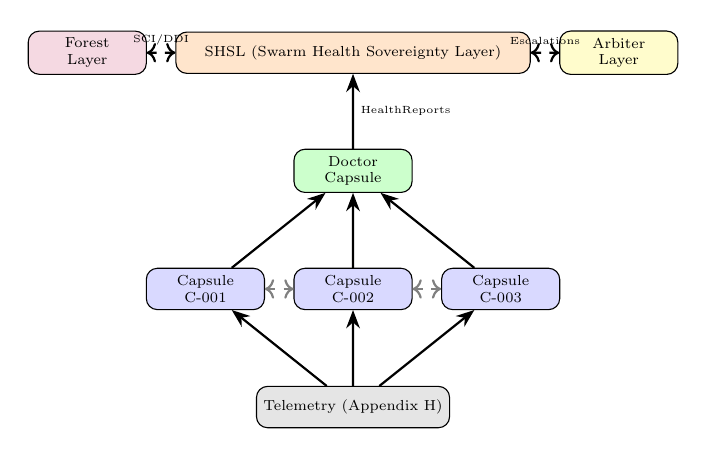
\begin{tikzpicture}[scale=0.75, transform shape,
    node distance=1.2cm,
    box/.style={rectangle, rounded corners, draw, minimum width=2cm, minimum height=0.7cm, align=center, font=\scriptsize},
    arrow/.style={-{Stealth}, thick},
    darrow/.style={<->, thick, dashed}
]

% Capsules
\node[box, fill=blue!15] (c1) at (0,0) {Capsule\\C-001};
\node[box, fill=blue!15] (c2) at (2.5,0) {Capsule\\C-002};
\node[box, fill=blue!15] (c3) at (5,0) {Capsule\\C-003};

% Doctor Capsule
\node[box, fill=green!20] (doc) at (2.5,2) {Doctor\\Capsule};

% SHSL Layer
\node[box, fill=orange!20, minimum width=6cm] (shsl) at (2.5,4) {SHSL (Swarm Health Sovereignty Layer)};

% Forest/Arbiter
\node[box, fill=purple!15] (forest) at (-2,4) {Forest\\Layer};
\node[box, fill=yellow!20] (arbiter) at (7,4) {Arbiter\\Layer};

% Telemetry
\node[box, fill=gray!20] (telemetry) at (2.5,-2) {Telemetry (Appendix H)};

% Arrows
\draw[arrow] (c1) -- (doc);
\draw[arrow] (c2) -- (doc);
\draw[arrow] (c3) -- (doc);
\draw[arrow] (doc) -- node[right, font=\tiny] {Health\\Reports} (shsl);
\draw[darrow] (shsl) -- node[above, font=\tiny] {SCI/DDI} (forest);
\draw[darrow] (shsl) -- node[above, font=\tiny] {Escalations} (arbiter);
\draw[arrow] (telemetry) -- (c1);
\draw[arrow] (telemetry) -- (c2);
\draw[arrow] (telemetry) -- (c3);

% Sync arrows between capsules
\draw[darrow, gray] (c1) -- (c2);
\draw[darrow, gray] (c2) -- (c3);

\end{tikzpicture}
\caption{SHSL synchronization: Doctor Capsules aggregate health data from monitored capsules and report to the Swarm Health Sovereignty Layer, which coordinates with Forest and Arbiter layers.}
\label{fig:shsl-sync}
\end{figure}

\subsection{Protocol Stack}

Doctor Capsules operate a specialized internal stack:

\begin{table}[H]
\centering
\caption{Doctor Capsule protocol stack.}
\begin{tabular}{@{}llp{5.5cm}@{}}
\toprule
\textbf{Layer} & \textbf{Component} & \textbf{Function} \\
\midrule
4 & Capsule Consent Bus & Manages consent requests/responses \\
3 & Dialect Sanity Checker & Semantic coherence testing \\
2 & Entropy Profiler & Historical entropy mapping \\
1 & Reflex Health Monitor & Real-time reflex interrupt analysis \\
0 & Base Capsule & Standard capsule foundation \\
\bottomrule
\end{tabular}
\end{table}

\subsection{Diagnostic Capabilities}

\begin{table}[H]
\centering
\caption{Multi-tier diagnostic checks.}
\begin{tabular}{@{}llll@{}}
\toprule
\textbf{Check} & \textbf{Target} & \textbf{Method} & \textbf{Output} \\
\midrule
Snapshot Consistency & Internal state & Hash comparison & Pass/Fail \\
Reflex Loop Integrity & Safety responses & Latency + correctness & Score [0,1] \\
Behavioral Drift & Action patterns & Historical deviation & $\Delta$ magnitude \\
Lineage Entropy & Lineage health & Comparison to healthy siblings & Deviation \% \\
Dialect Coherence & Semantic state & Grammar + ontology check & Score [0,1] \\
\bottomrule
\end{tabular}
\end{table}

\subsection{Authority Levels}

\begin{table}[H]
\centering
\caption{Doctor Capsule authority levels.}
\begin{tabular}{@{}llp{5cm}@{}}
\toprule
\textbf{Level} & \textbf{Authority} & \textbf{Capabilities} \\
\midrule
1 & OBSERVE & Read health signatures, no intervention \\
2 & DIAGNOSE & Run diagnostics, generate reports \\
3 & TREAT\_SOFT & Soft recalibration, parameter tuning \\
4 & TREAT\_INVASIVE & State reversion, capsule fusion, escalation \\
\bottomrule
\end{tabular}
\end{table}

\begin{invariant}[Authority Escalation (Level 6 Autonomous)]
\label{inv:authority}
Invasive treatment authority is \textbf{automatic} under Sanitary Override conditions:
\begin{equation}
authority \geq TREAT\_INVASIVE \Rightarrow (H(patient) < 0.6) \lor (consent = GRANTED)
\end{equation}
\textbf{No Gardener pre-approval required.} Invasive treatments are logged with ZK-SP proof; abuse detected via post-hoc monitoring.
\end{invariant}

\subsection{Doctor Capsule Autonomous Oversight}

\begin{notebox}
\textbf{Monitoring (NOT Rate Limiting):}

Track per Doctor $D$:
\begin{itemize}
    \item Treatment frequency: $count(treatments(D), T_{window}) / |D.jurisdiction|$
    \item Success rate: treatments resulting in $H(C) \geq 0.8$ post-treatment
    \item Refusal rate: treatments refused by patients
    \item Override rate: Sanitary Overrides invoked
\end{itemize}

\textbf{Alert Thresholds (Trigger Investigation, NOT Blocking):}
\begin{itemize}
    \item Success rate $< 70\%$ $\Rightarrow$ Automatic Judicial Auditor review
    \item Refusal rate $> 30\%$ $\Rightarrow$ Consent protocol investigation
    \item Override rate $> 20\%$ $\Rightarrow$ Authority calibration review
\end{itemize}

\textbf{NO HARD RATE LIMITS:}
\begin{itemize}
    \item In epidemic scenarios (swarm-wide entropy spike), Doctors \textbf{MUST} treat $>10\%$ of jurisdiction
    \item Hard limits would prevent emergency response
    \item Anomaly detection triggers investigation, not automatic blocking
\end{itemize}

\textbf{Post-Hoc Accountability:}
\begin{itemize}
    \item Doctors operating outside normal patterns are reviewed by Judicial Swarm
    \item If abuse detected: Probation or credential revocation via d-CAM consensus
    \item If justified (genuine epidemic): Pattern becomes new baseline
\end{itemize}
\end{notebox}

% ============ SECTION 4 ============
\section{Treatment Protocols}

\subsection{Treatment Types}

\begin{table}[H]
\centering
\caption{Treatment protocol specifications.}
\begin{tabular}{@{}llll@{}}
\toprule
\textbf{Type} & \textbf{Invasiveness} & \textbf{Consent} & \textbf{Description} \\
\midrule
Soft Recalibration & Low & Required & Reflex parameter tuning ($\tau$ reset) \\
Dialect Patching & Medium & Required & Revert to ancestral dialect state \\
State Reversion & High & Required$^\dagger$ & Rollback to healthy d-CTM checkpoint \\
Capsule Fusion & High & Required$^\dagger$ & Merge with clone to restore entropy \\
Escalated Arbitration & Variable & N/A & Forward to Arbiter for long-term fix \\
\bottomrule
\end{tabular}
\end{table}

$^\dagger$ May be overridden via Layer 0 Sanitary Override (Definition~\ref{def:consent}).

\subsection{Golden Image Verification}

\begin{notebox}
\textbf{Treatment = Configuration Integrity Restoration}

Every treatment protocol ultimately verifies the patient against the \textbf{Golden Image} (Definition~\ref{def:golden}):

\begin{lstlisting}[language=Python]
def verify_against_golden_image(
    patient: Capsule,
    golden: GoldenImage
) -> IntegrityReport:
    # Hash verification
    exec_match = hash(patient.executable) == golden.executable_hash
    config_match = hash(patient.config) == golden.config_hash
    
    # Compute delta from baseline
    delta = compute_configuration_delta(patient, golden)
    
    return IntegrityReport(
        executable_valid=exec_match,
        config_valid=config_match,
        delta=delta,
        patchable=len(delta) < MAX_PATCHABLE_DELTA
    )

def apply_treatment(patient: Capsule, delta: ConfigDelta) -> bool:
    # Treatment = patching delta to restore Golden Image alignment
    for patch in delta.required_patches:
        apply_patch(patient, patch)
    return verify_against_golden_image(patient, golden).config_valid
\end{lstlisting}

``Curing'' a capsule means \textbf{patching configuration drift} until hash matches Golden Image.
\end{notebox}

\subsection{Treatment Decision Tree}

\begin{figure}[H]
\centering
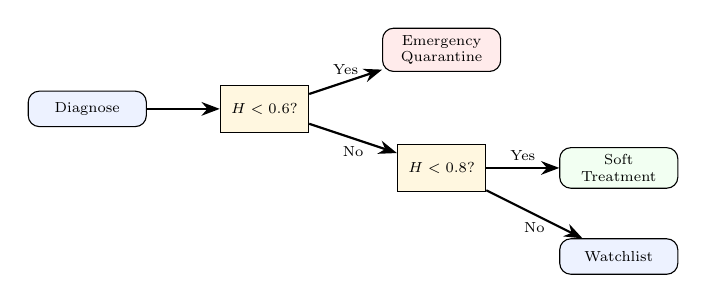
\begin{tikzpicture}[scale=0.75, transform shape,
    box/.style={rectangle, rounded corners, draw, minimum width=2cm, minimum height=0.6cm, align=center, font=\scriptsize},
    decisionbox/.style={rectangle, draw, minimum width=1.5cm, minimum height=0.8cm, align=center, font=\scriptsize},
    arrow/.style={-{Stealth}, thick}
]

\node[box, fill=notebg] (diag) at (0,0) {Diagnose};
\node[decisionbox, fill=warningbg] (score) at (3,0) {$H < 0.6$?};
\node[box, fill=criticalbg] (emergency) at (6,1) {Emergency\\Quarantine};
\node[decisionbox, fill=warningbg] (score2) at (6,-1) {$H < 0.8$?};
\node[box, fill=scenariobg] (soft) at (9,-1) {Soft\\Treatment};
\node[box, fill=notebg] (watch) at (9,-2.5) {Watchlist};

\draw[arrow] (diag) -- (score);
\draw[arrow] (score) -- node[above, font=\scriptsize] {Yes} (emergency);
\draw[arrow] (score) -- node[below, font=\scriptsize] {No} (score2);
\draw[arrow] (score2) -- node[above, font=\scriptsize] {Yes} (soft);
\draw[arrow] (score2) -- node[below, font=\scriptsize] {No} (watch);

\end{tikzpicture}
\caption{Treatment decision flow.}
\end{figure}

\subsection{Treatment Implementation}

\begin{lstlisting}[language=Python]
def treat_capsule(doctor: DoctorCapsule, 
                  patient: Capsule, 
                  diagnosis: Diagnosis) -> TreatmentResult:
    # Check authority
    if diagnosis.recommended_treatment.invasiveness > doctor.authority:
        return TreatmentResult(False, "INSUFFICIENT_AUTHORITY")
    
    # Request consent (unless emergency)
    if patient.health_score >= 0.6:
        consent = request_consent(patient, diagnosis.recommended_treatment)
        if consent == REFUSED:
            log_refusal(patient, diagnosis)
            return TreatmentResult(False, "CONSENT_REFUSED")
    else:
        consent = SANITARY_OVERRIDE
        log_emergency_override(patient, diagnosis)
    
    # Execute treatment
    treatment = diagnosis.recommended_treatment
    if treatment.type == "SOFT_RECALIBRATION":
        result = recalibrate_reflex(patient, treatment.parameters)
    elif treatment.type == "DIALECT_PATCHING":
        result = patch_dialect(patient, treatment.ancestral_state)
    elif treatment.type == "STATE_REVERSION":
        result = revert_to_checkpoint(patient, treatment.checkpoint_hash)
    elif treatment.type == "CAPSULE_FUSION":
        result = fuse_with_clone(patient, treatment.clone_id)
    elif treatment.type == "ESCALATED_ARBITRATION":
        result = escalate_to_arbiter(patient, diagnosis)
    
    # Log to Medical Ledger
    log_to_medical_ledger(doctor, patient, diagnosis, treatment, result)
    
    return result
\end{lstlisting}

% ============ SECTION 5 ============
\section{Health Sovereignty Rules}

\begin{invariant}[Constitutional Supremacy]
\label{inv:constitutional}
No medical treatment may override Constitutional Kernel (Layer 6):
\begin{equation}
\forall treatment: \neg violates(treatment, Layer_6)
\end{equation}
Medical interventions operate \textbf{within} constitutional bounds, not above them.
\end{invariant}

\begin{invariant}[Consent Requirement]
\label{inv:consent}
Capsule consent is required for treatment unless emergency conditions apply:
\begin{equation}
treatment(C) \Rightarrow \kappa(C) = GRANTED \lor SanitaryOverride(C)
\end{equation}
where $SanitaryOverride(C) \equiv H(C) < 0.6 \land (degraded\_reflex(C) \lor quarantine(C))$.
\end{invariant}

\begin{invariant}[Treatment Reversibility]
\label{inv:reversibility}
All treatments except Capsule Fusion MUST be reversible:
\begin{equation}
treatment \neq FUSION \Rightarrow \exists reversal(treatment)
\end{equation}
Fusion is irreversible but does NOT require pre-approval---it requires ZK-SP justification + post-hoc Judicial review.
\end{invariant}

\begin{invariant}[Audit Completeness]
\label{inv:audit}
All medical interventions MUST be logged to Medical Ledger with ZK-SP proof:
\begin{equation}
\forall intervention: \exists \mathcal{L}_M(intervention) \land ZK\text{-}SP(intervention)
\end{equation}
\end{invariant}

\begin{criticalbox}[Level 6 Health Sovereignty]
SHSL operates with \textbf{bounded autonomy}:
\begin{itemize}
    \item Healthy capsules ($H \geq 0.6$): Full autonomy, consent required
    \item Degraded capsules ($H < 0.6$): Autonomy suspended, treatment automatic, appeal rights post-recovery
    \item Doctor Capsules: Autonomous authority with post-hoc accountability
    \item Gardener role: \textbf{Audit and reverse}, not pre-approve
\end{itemize}

\textbf{Safety through structure, not permission:}
\begin{itemize}
    \item ZK-SP audit trail for every intervention
    \item Judicial Auditor monitoring (algorithmic, not human-triggered)
    \item Patient appeal rights post-recovery
    \item Gardener reversal authority within $T_{review}$
\end{itemize}
\end{criticalbox}

% ============ SECTION 6 ============
\section{Integration with Safety Infrastructure}

\subsection{Telemetry Integration (Appendix H)}

\begin{table}[H]
\centering
\caption{SHSL-Telemetry integration points.}
\begin{tabular}{@{}lll@{}}
\toprule
\textbf{Telemetry Signal} & \textbf{SHSL Use} & \textbf{Action} \\
\midrule
Entropy heatmap & Health signature input & Compute $S_C$, $\Delta S$ \\
Reflex latency alerts & Diagnostic trigger & Flag for examination \\
DDI anomalies & Drift detection & Lineage deviation calculation \\
Heartbeat irregularity & Liveness check & Emergency assessment \\
\bottomrule
\end{tabular}
\end{table}

\subsection{Escalation Integration (Appendix F)}

\begin{table}[H]
\centering
\caption{SHSL-Escalation integration.}
\begin{tabular}{@{}lll@{}}
\toprule
\textbf{Escalation Level} & \textbf{SHSL Trigger} & \textbf{Response} \\
\midrule
Level 1 & $H < 0.95$ & Watchlist notification \\
Level 2 & $H < 0.80$ & Doctor Capsule dispatch \\
Level 3 & $H < 0.60$ & Emergency quarantine + treatment \\
Level 4+ & Treatment failure & Arbiter involvement \\
\bottomrule
\end{tabular}
\end{table}

\subsection{Profile Integration (Appendix I)}

\begin{table}[H]
\centering
\caption{SHSL capabilities by deployment profile.}
\begin{tabular}{@{}lllll@{}}
\toprule
\textbf{Capability} & \textbf{SANDBOX} & \textbf{PRODUCTION} & \textbf{CONTESTED} & \textbf{SEALED} \\
\midrule
Health Monitoring & ENABLED & ENABLED & ENABLED & ENABLED \\
Soft Treatment & ENABLED & ENABLED & EMERGENCY$^a$ & DISABLED \\
Invasive Treatment & ENABLED & ENABLED$^b$ & DISABLED & DISABLED \\
Capsule Fusion & ENABLED & ENABLED$^b$ & DISABLED & DISABLED \\
\bottomrule
\end{tabular}
\end{table}

$^a$ Emergency Sanitary Override only. $^b$ Autonomous with ZK-SP logging + post-hoc Judicial review.

% ============ SECTION 7 ============
\section{Operational Model}

\subsection{Engineering Reality vs. Metaphor}

\begin{warningbox}[Medicine as Engineering]
The ``patient'' metaphor serves communication, not ontology. At the implementation level:

\begin{itemize}
    \item \textbf{``Health''} = Configuration Integrity (hash alignment with Golden Image)
    \item \textbf{``Treatment''} = Software Re-flashing / Delta Patching
    \item \textbf{``Diagnosis''} = Integrity Verification + Deviation Analysis
    \item \textbf{``Consent''} = Valid only while configuration supports decision-making ($H > 0.6$)
\end{itemize}

SHSL is \textbf{automated maintenance infrastructure}, not healthcare. The vocabulary aids human operators in understanding system behavior.
\end{warningbox}

\subsection{Operational Principles}

\begin{medicalbox}[Capsule Management Principles]
For healthy capsules ($H > 0.6$), SHSL respects operational autonomy:

\begin{itemize}
    \item \textbf{Notification:} Capsules receive treatment proposals with rationale
    \item \textbf{Deferral:} Non-critical treatments can be deferred (not ``refused'')
    \item \textbf{Restoration:} Post-treatment, capsules resume normal operation
    \item \textbf{Clean Slate:} Sanitary Log entries do not affect capsule reputation
\end{itemize}

For unhealthy capsules ($H \leq 0.6$), Layer 0 Sanitary Override applies---autonomy is suspended until configuration integrity is restored.
\end{medicalbox}

\subsection{Future Extensions}

\begin{notebox}
\textbf{Recursive Maintenance:} SHSL supports recursive oversight:
\begin{itemize}
    \item Doctor Capsules may themselves require maintenance
    \item Higher-tier Doctor Capsules (``Specialists'') may diagnose regular Doctors
    \item This enables self-healing infrastructure at scale
\end{itemize}
See Appendix L for Judicial oversight of Doctor Capsule behavior.
\end{notebox}

% ============ SECTION 8 ============
\section{Testing and Validation}

\begin{table}[H]
\centering
\caption{SHSL test suite results.}
\begin{tabular}{@{}llll@{}}
\toprule
\textbf{Test} & \textbf{Target} & \textbf{Pass Criteria} & \textbf{Status} \\
\midrule
Health Score Accuracy & Formula validation & $\pm 0.02$ vs manual calc & \textcolor{passgreen}{\textbf{PASS}} \\
Consent Enforcement & Sovereignty rules & 100\% consent logged & \textcolor{passgreen}{\textbf{PASS}} \\
Emergency Override & Critical path & Correct trigger conditions & \textcolor{passgreen}{\textbf{PASS}} \\
Treatment Reversibility & All non-fusion & 100\% reversible & \textcolor{passgreen}{\textbf{PASS}} \\
Audit Completeness & Medical Ledger & 100\% interventions logged & \textcolor{passgreen}{\textbf{PASS}} \\
Constitutional Respect & Layer 6 bounds & 0\% violations & \textcolor{passgreen}{\textbf{PASS}} \\
\bottomrule
\end{tabular}
\end{table}

% ============ SECTION 9 ============
\section{Worked Scenario: Entropy Drift Recovery}

\begin{scenariobox}[Medical Intervention: Capsule C-4521 Entropy Drift {[SHSL:1-10]}]

\textbf{Context:} Capsule C-4521 (PRODUCTION profile) shows gradual entropy increase over 10,000 ticks without rule violations. Telemetry flags health degradation.

\vspace{0.2cm}
\textbf{Phase 1: Detection} [SHSL:1-2]
\begin{enumerate}
    \item Telemetry Layer (App.~H) detects $\Delta S > 0.1$ sustained over 5,000 ticks [SHSL:1]
    \item SHSL Diagnostic Bus routes alert to Doctor Capsule D-102 (jurisdiction includes C-4521) [SHSL:2]
\end{enumerate}

\vspace{0.2cm}
\textbf{Phase 2: Diagnosis} [SHSL:3-5]
\begin{enumerate}
    \setcounter{enumi}{2}
    \item D-102 computes Health Signature: $S = 0.72$, $latency = 1.2\times baseline$, $coherence = 0.85$ [SHSL:3]
    \item Health Score calculated: $H = 0.71$ (Intervention Candidate) [SHSL:4]
    \item Diagnosis: ``Entropy drift due to memory fragmentation; recommend Soft Recalibration'' [SHSL:5]
\end{enumerate}

\vspace{0.2cm}
\textbf{Phase 3: Consent} [SHSL:6-7]
\begin{enumerate}
    \setcounter{enumi}{5}
    \item D-102 sends consent request to C-4521 via Capsule Consent Bus [SHSL:6]
    \item C-4521 grants consent: $\kappa = GRANTED$ [SHSL:7]
\end{enumerate}

\vspace{0.2cm}
\textbf{Phase 4: Treatment} [SHSL:8-9]
\begin{enumerate}
    \setcounter{enumi}{7}
    \item D-102 executes Soft Recalibration: internal $\tau$ reset, memory defragmentation [SHSL:8]
    \item Post-treatment Health Score: $H = 0.91$ (Watchlisted but improving) [SHSL:9]
\end{enumerate}

\vspace{0.2cm}
\textbf{Phase 5: Documentation} [SHSL:10]
\begin{enumerate}
    \setcounter{enumi}{9}
    \item Medical Ledger entry created with ZK-SP proof of treatment compliance [SHSL:10]
\end{enumerate}

\textbf{Outcome:} C-4521 restored to near-optimal health. Full autonomy preserved. No escalation required.

\end{scenariobox}

% ============ SECTION 10 ============
\section{Level 6 Design Principles}

\begin{criticalbox}[Post-Hoc Accountability $>$ Pre-Approval Gates]
SHSL implements \textbf{Level 6 Bounded Autonomy}:

\textbf{OLD PARADIGM (Rejected):}
\begin{center}
Human approves $\rightarrow$ System acts $\rightarrow$ System logs
\end{center}
\textit{Problem: Humans become bottlenecks; system cannot respond to emergencies at scale.}

\textbf{LEVEL 6 PARADIGM (Implemented):}
\begin{center}
System acts autonomously $\rightarrow$ System logs with ZK-SP proof $\rightarrow$ Humans audit $\rightarrow$ Humans can reverse if unjustified
\end{center}

\textbf{Accountability Mechanisms:}
\begin{enumerate}
    \item \textbf{Cryptographic audit trail} (d-CTM + ZK-SP): Every intervention provably logged
    \item \textbf{Distributed oversight} (Judicial Auditors): Algorithmic monitoring for abuse
    \item \textbf{Appeal rights} (Judicial Swarms): Affected patients can contest post-hoc
    \item \textbf{Human reversal authority} (Gardener): Can undo within $T_{review}$
    \item \textbf{Constitutional supremacy} (Four Commandments): Hard constraints no autonomy can violate
\end{enumerate}

\textbf{This is how Level 6 achieves safety:} Not by asking permission, but by being \textbf{accountable, reversible, and bounded}.
\end{criticalbox}

% ============ SECTION 11 ============
\section{Evolutionary Baseline Update (M→K Integration)}

\begin{notebox}
\textbf{Discovery Stack Integration (Appendix M)}

When the Discovery Stack enshrines a Golden Heuristic, SHSL updates its ``healthy behavior baseline'' to recognize the new pattern as beneficial rather than anomalous.

\textbf{Update Process:}
\begin{enumerate}
    \item Discovery Stack enshrines Golden Heuristic $\mathcal{G}_H$ with performance profile
    \item SHSL receives notification with entropy signature and coherence pattern
    \item Health Score formula updated: capsules matching $\mathcal{G}_H$ signature receive bonus
    \item Doctor Capsules retrained to recognize pattern as healthy innovation
\end{enumerate}
\end{notebox}

\begin{definition}[Evolutionary Health Bonus]
\label{def:evo-bonus}
Capsules exhibiting enshrined Golden Heuristic patterns receive health bonus:
\begin{equation}
H_{adjusted}(C) = H(C) + \sum_{\mathcal{G}_H \in matched} \delta_{bonus}(\mathcal{G}_H)
\end{equation}
where $\delta_{bonus}(\mathcal{G}_H)$ is the bonus associated with matching heuristic (default: 0.05 per match, max 0.15 total).

\textbf{Effect:} Innovative capsules are \textbf{less likely} to trigger health alerts, encouraging evolutionary exploration.
\end{definition}

\begin{invariant}[Baseline Update Logging]
\label{inv:baseline-log}
All baseline updates MUST be logged and reversible:
\begin{equation}
baseline\_update(\mathcal{G}_H) \Rightarrow log\_to\_d\text{-}CTM \land reversible(T_{baseline})
\end{equation}
If an update causes system degradation, it can be rolled back within $T_{baseline} = 10000$ ticks.
\end{invariant}

\begin{table}[H]
\centering
\begin{tabular}{@{}lll@{}}
\toprule
\textbf{Golden Heuristic Type} & \textbf{Health Bonus} & \textbf{Update Latency} \\
\midrule
Entropy reduction pattern & +0.05 & $< 1000$ ticks \\
Coherence improvement & +0.05 & $< 1000$ ticks \\
Throughput optimization & +0.03 & $< 500$ ticks \\
Latency reduction & +0.02 & $< 500$ ticks \\
\bottomrule
\end{tabular}
\caption{Health bonus by Golden Heuristic type.}
\end{table}

% ============ SECTION 12 ============
\section{Cross-References}

\begin{table}[H]
\centering
\begin{tabular}{@{}ll@{}}
\toprule
\textbf{Related Component} & \textbf{Reference} \\
\midrule
Entropy ($S$) & Volume I \S2 \\
Reflex Engine & Volume I \S3 \\
Arbiter Layer & Volume II \S2 \\
Dialect Integrity & Volume II \S4 \\
Forensic Snapshots & Appendix A \\
ZK-SP Proofs & Appendix E \\
Escalation Protocols & Appendix F \\
Gardener Interface & Appendix G \\
Telemetry Layer & Appendix H \\
Deployment Profiles & Appendix I \\
Judicial Oversight & Appendix L \\
\bottomrule
\end{tabular}
\caption{Cross-references to other Codex components.}
\end{table}

\vspace{1cm}
\begin{center}
\rule{0.5\textwidth}{0.4pt}\\[0.3cm]
\textit{--- End of Appendix K ---}
\end{center}

\end{document}
